\section{Performance evaluation}

We evaluate the computational overhead introduced by DSphinx and by the destination-bound credential mechanism, as well as their scalability with respect to the main system parameters. 
We implemented a Python prototype\footnote{\artifact} to compare three configurations: DSphinx with credentials, vanilla DSphinx, and the original Sphinx packet construction of Danezis, which we use as a baseline.

All measurements reported in this section were obtained on a 13th Gen Intel Core i7-13700HX CPU running at 3.70 GHz. 
Unless otherwise stated, the benchmark simulates a network of 50 clients, 50 mixnodes, and 50 credential authorities, with each client sending five messages to itself.

\subsection{Parameter sensitivity}

We first perform a preliminary sensitivity analysis to identify the parameters that most strongly affect the computational cost of each protocol phase. 
For each phase and parameter $x$, we fit the empirical power-law model
$
T(x) \propto x^\lambda
$
using a linear regression in log-log space. The exponent $\lambda$ characterizes the observed scaling, with values close to $0$, $1$, and $2$ indicating approximately constant, linear, and quadratic behavior, respectively. The coefficient of determination $R^2$ indicates the goodness of fit.

As shown in Figure~\ref{im:scaling}, the clearest dependencies are observed for the path length $m$ and reconstruction threshold $k$.
Header Construction exhibits near-quadratic scaling with $m$ ($\lambda=2.03$, $R^2=0.88$), while Setup and Credential Issuance exhibit approximately linear-to-superlinear scaling with the threshold ($\lambda=1.32$, $R^2=0.86$ and $\lambda=1.03$, $R^2=0.71$, respectively). 
The remaining parameters show weak fits and provide little evidence of consistent scaling.
We therefore focus the remainder of the evaluation on the path length $m$ and reconstruction threshold $k$.

\begin{figure}
    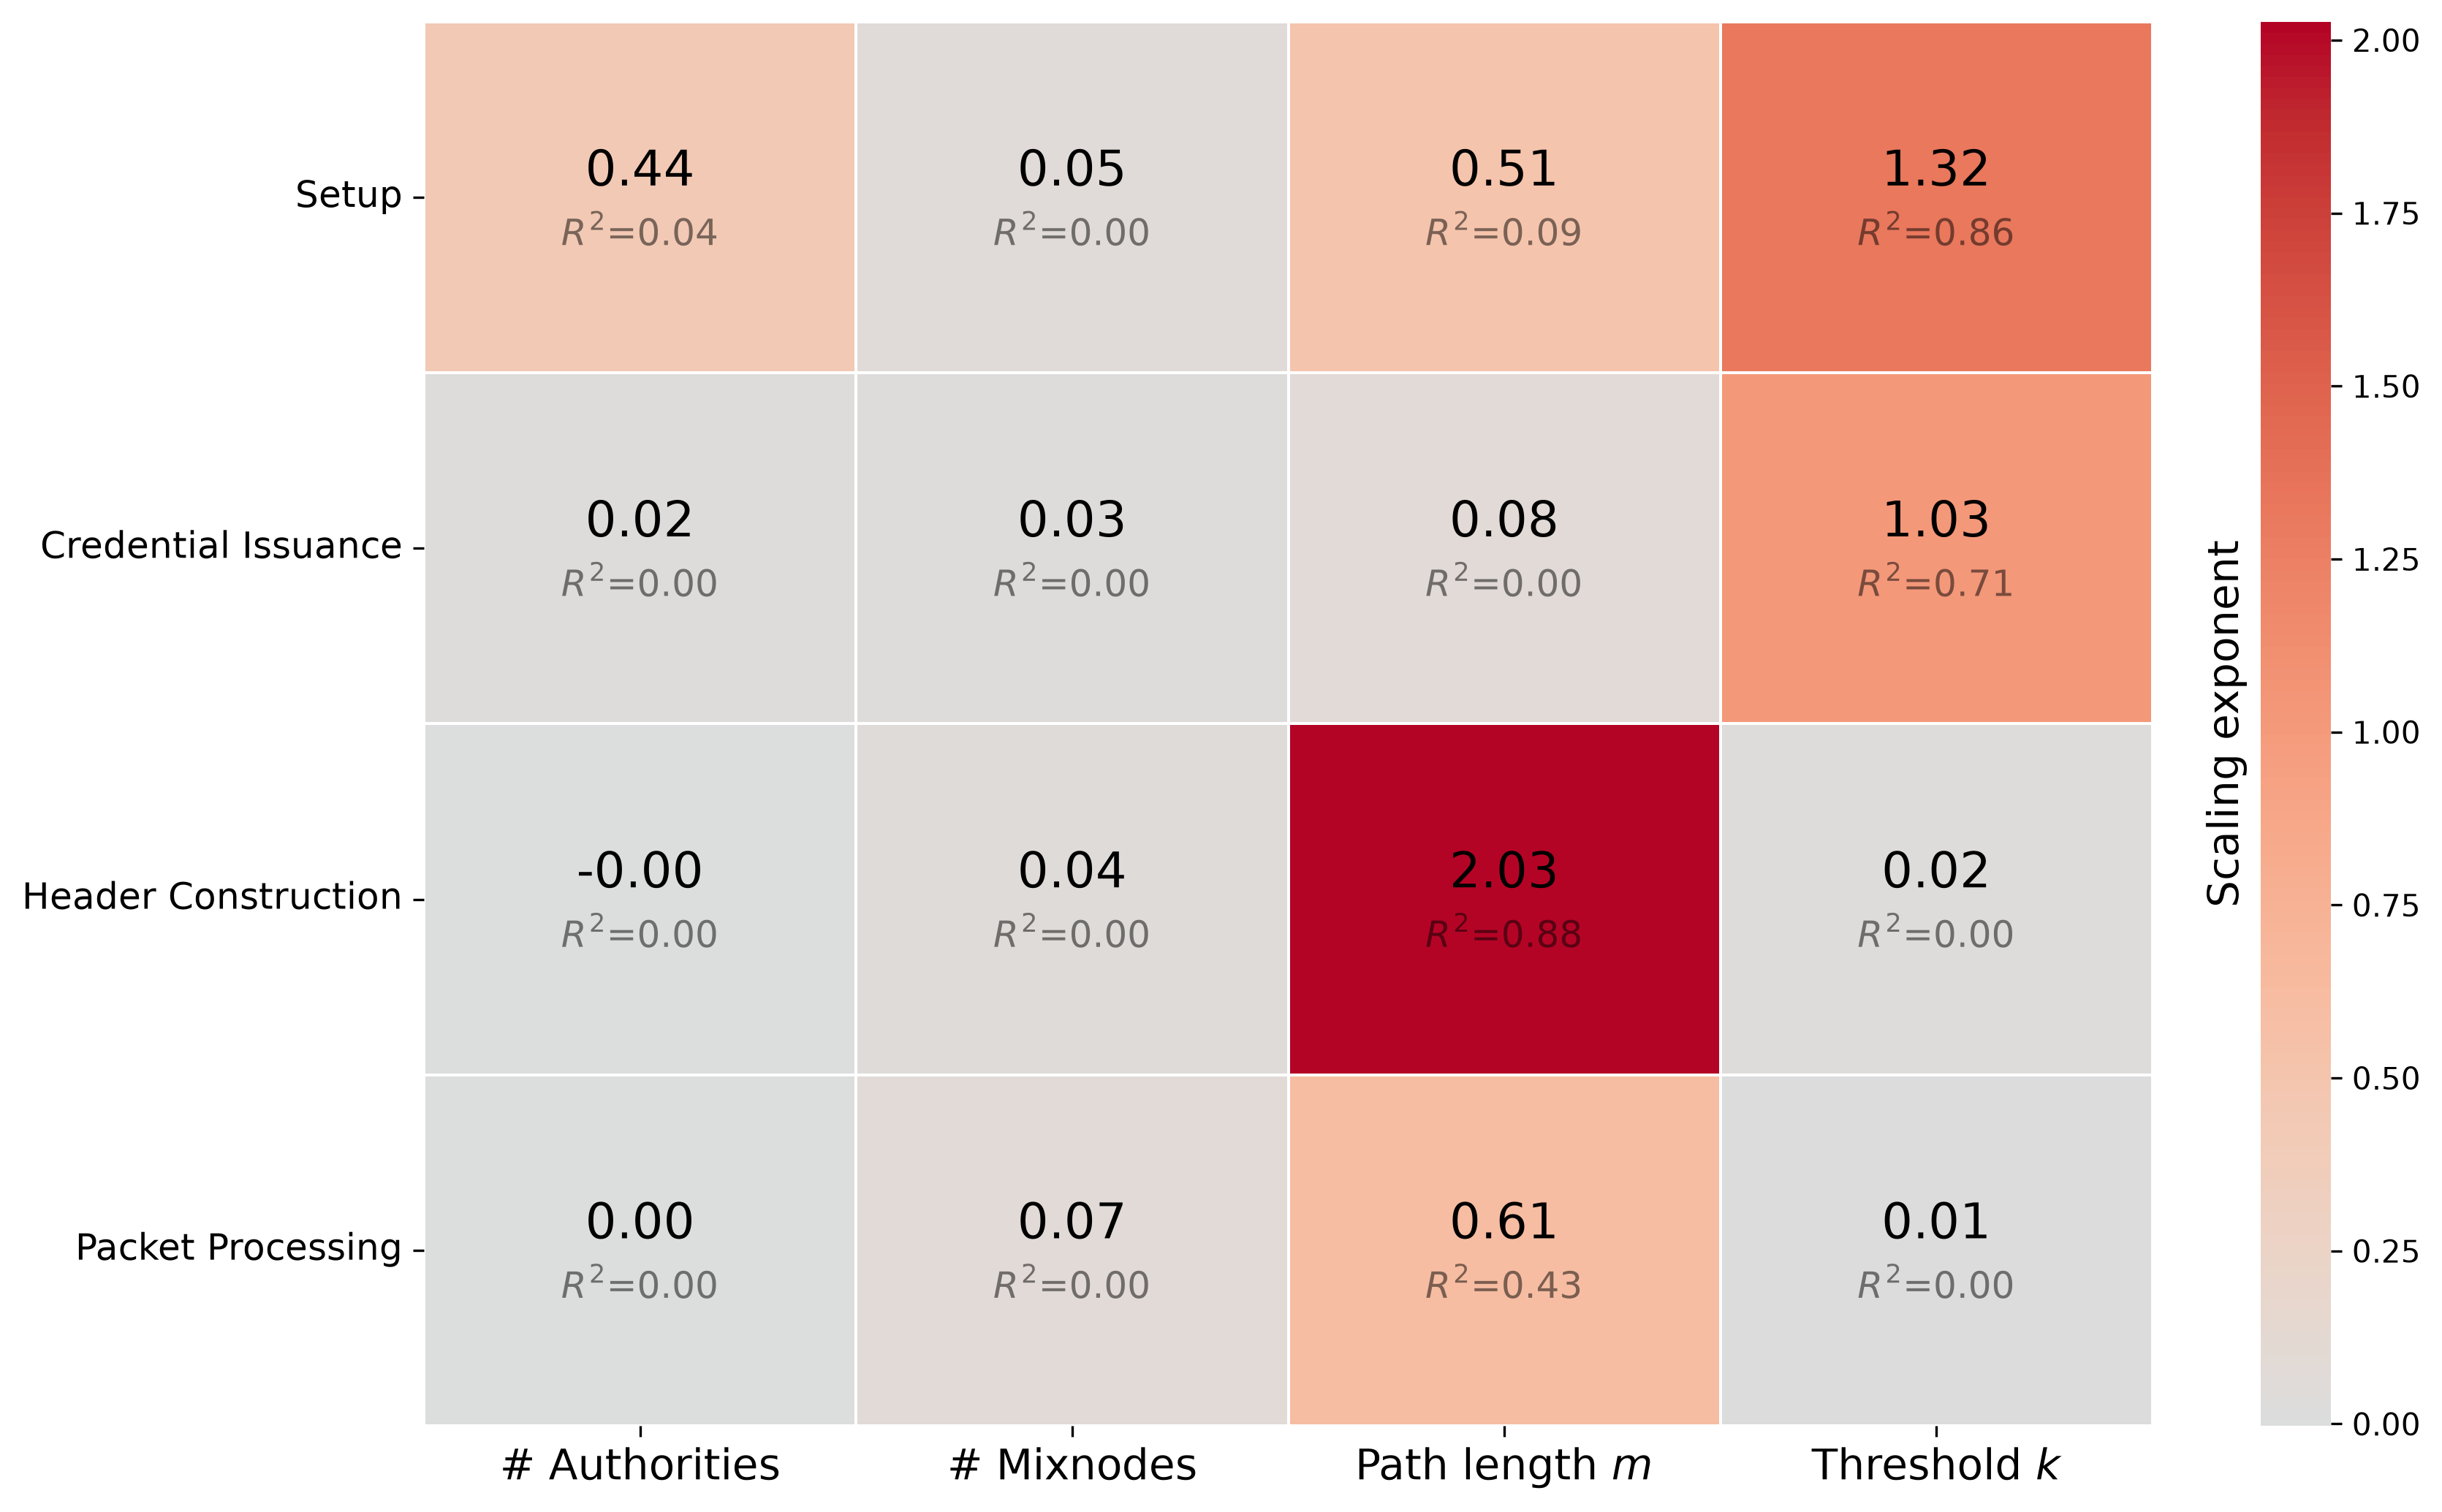
\includegraphics[width=\linewidth]{Images/scaling.png}
    \caption{
    Empirical scaling of the protocol phases with respect to the main system parameters.
    Each cell shows the scaling exponent $\lambda$, with its goodness of fit $R^2$.
    }
    \label{im:scaling}
\end{figure}


\subsection{Packet construction and processing}

For the first experiment, we compare the computational cost of packet's header generation at the client and packet processing at a mixnode for DSphinx with credential, vanilla DSphinx, and the Sphinx baseline. 
We vary the path length $m$ from 3 to 7 hops with a fixed reconstruction threshold $k=20$.
This range follows the maximum path length supported by the original Sphinx implementation used as our baseline. 
The results are shown in Figure~\ref{im:computation_time}.

From the client perspective, DSphinx requires approximately two to three times more computation than the Sphinx baseline for header generation.
Nevertheless, the absolute cost remains below 12 ms for a seven-hop path.
Adding the credential introduces only a small additional cost, primarily associated with the credential-binding operation of Equation~\eqref{eq:header_bound_credential}.

At the mixnode, vanilla DSphinx introduces an additional cost of approximately 1 ms compared with Sphinx, while credential verification adds approximately 2 ms. 
Although this corresponds to an absolute overhead of less than 3 ms, the relative overhead is substantial because baseline Sphinx packet processing remains approximately constant at 0.2 ms in our experiment. 
Therefore the credential version requires approximately 10-15 times more computation than the Sphinx baseline. 
The dominant source of this additional cost is the two pairing operations required for credential verification in Equation~\eqref{eq:credential_verification}.

\begin{figure}
    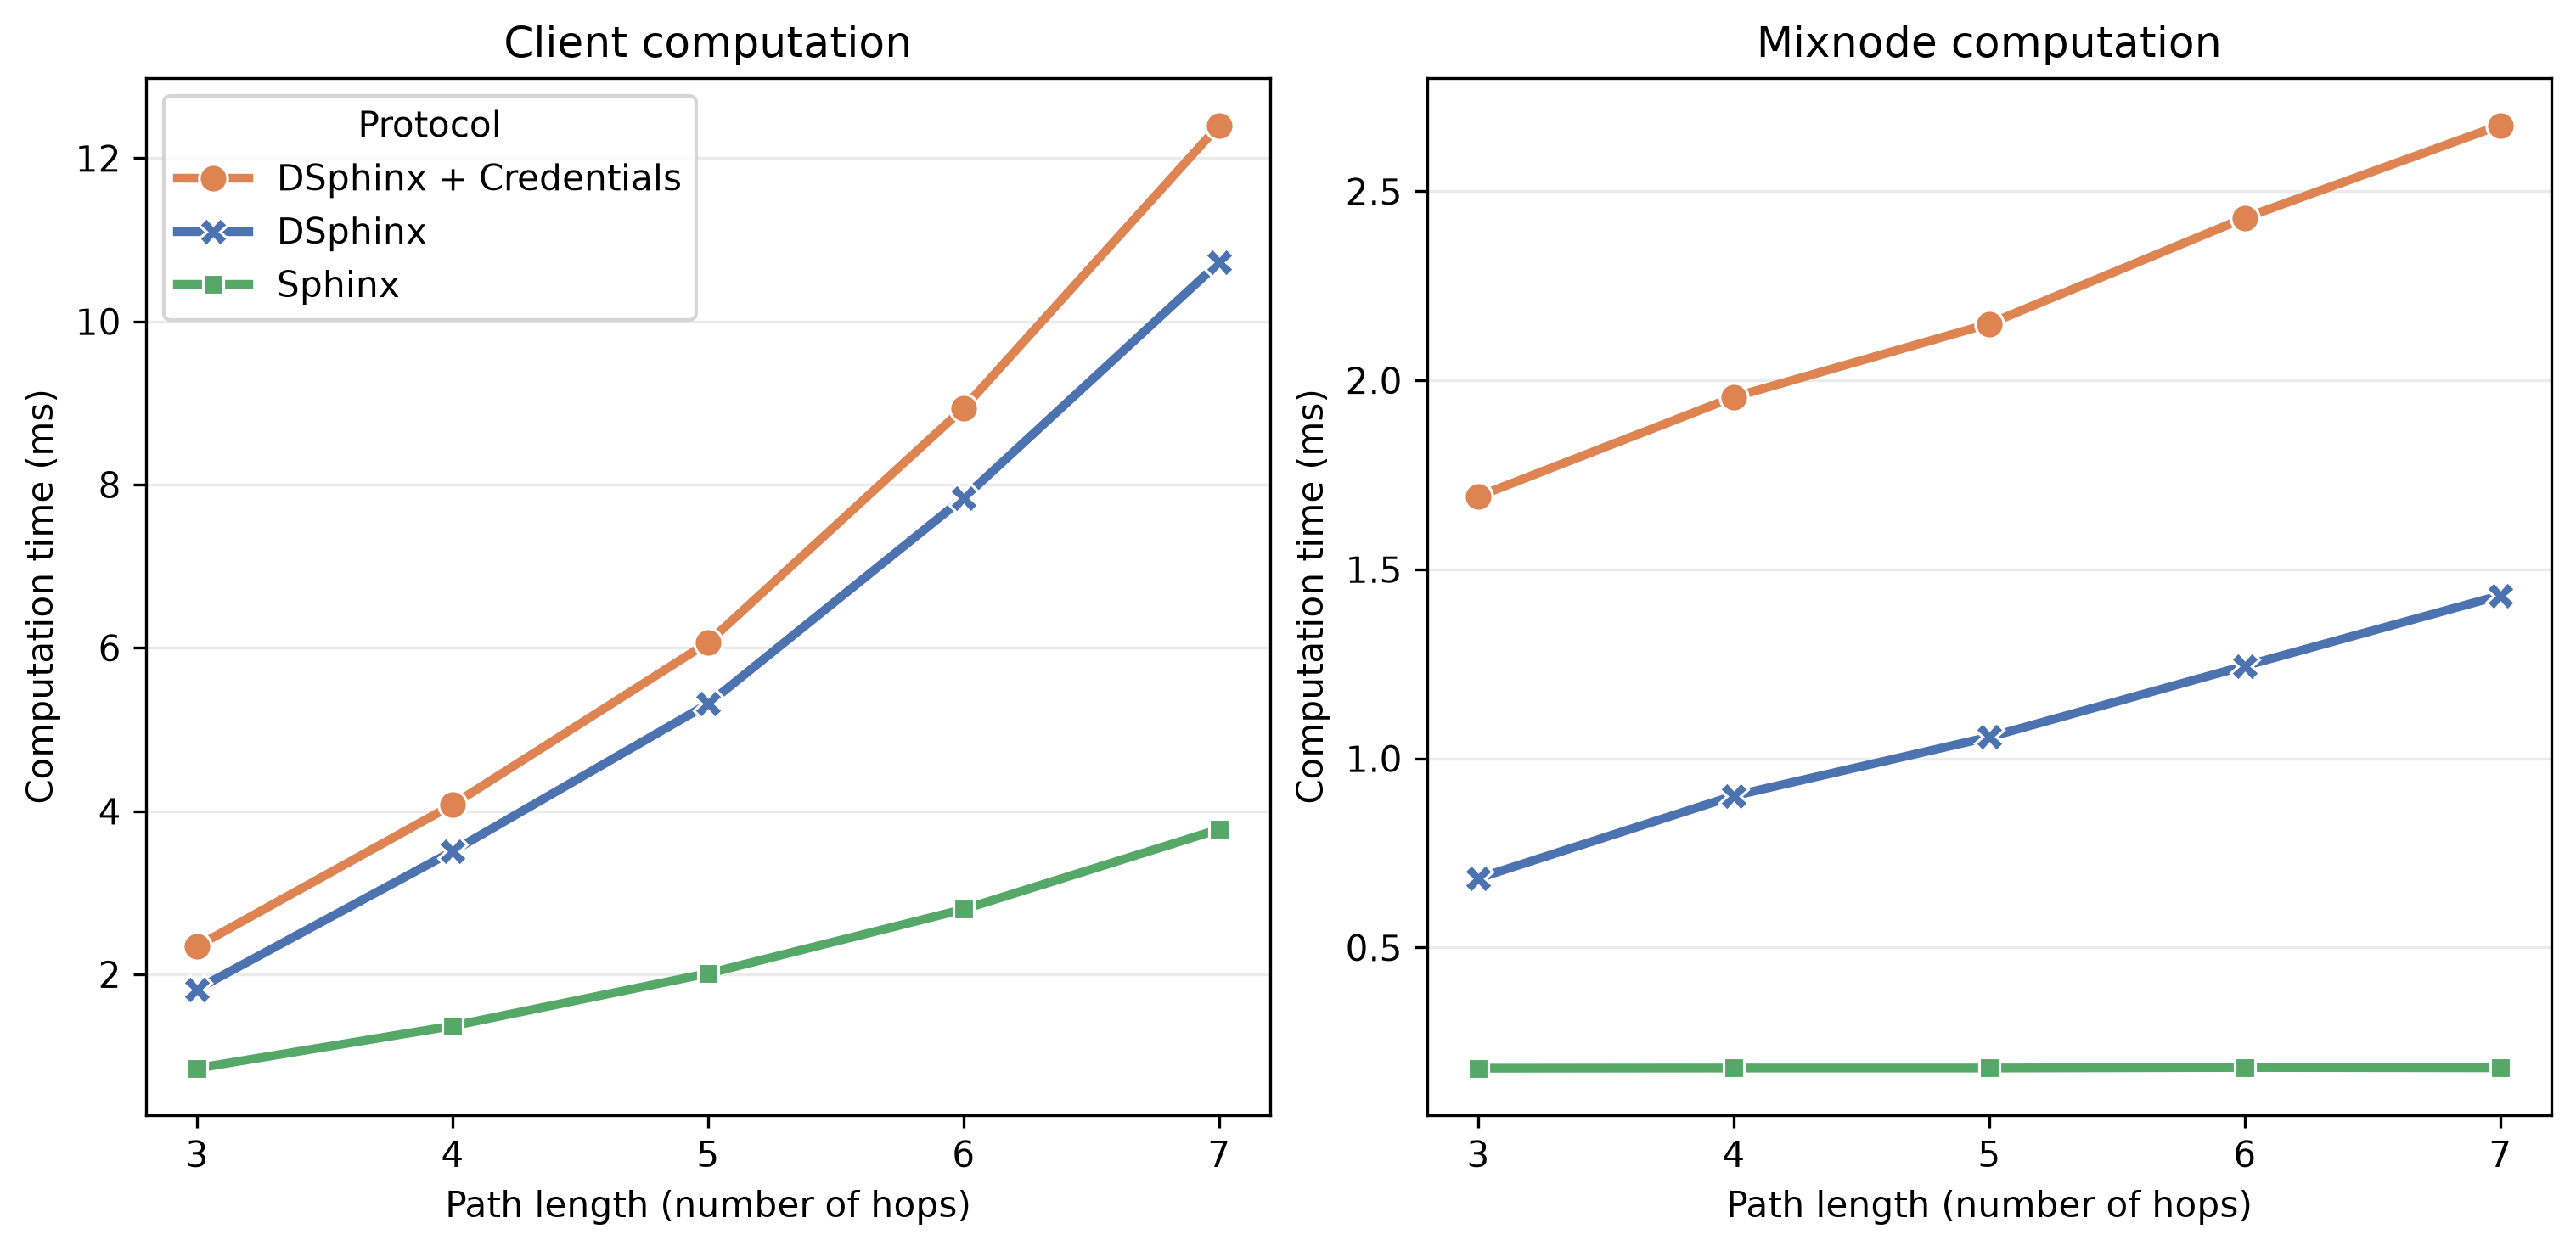
\includegraphics[width=\linewidth]{Images/computation_time.png}
    \caption{Computation time for packet's header generation at the client and packet processing at a mixnode as a function of the path length $m$, ranging from 3 to 7 hops.}
    \label{im:computation_time}
\end{figure}

\subsection{Setup and credential issuance}

We next evaluate the additional procedures required by our scheme, the system setup and credential issuance. 
The setup is performed once during system initialization, whereas credential issuance is performed by a client for each destination for which it requires a destination-bound credential.
As indicated by Figure~\ref{im:scaling}, the reconstruction threshold $k$ is the dominant parameter for these operations. 
We therefore vary $k$ while fixing the path length to $m=5$. 
Figure~\ref{im:setup_time} presents the corresponding execution times.

The setup procedure is the most computationally expensive operation in our scheme. 
For $k=50$, it requires up to approximately 500 ms in our prototype. 
This cost is incurred only once during initialization.
The measured cost is primarily attributed to the Lagrange-polynomial interpolation of degree $k-1$ used to authenticate the public parameters.

Credential issuance requires approximately 10-70 ms at the client, including the request and the aggregation of the partial credentials returned by the authorities. 
In this experiment, the computational cost at an authority is negligible because we consider only the basic credential-issuance operation and do not include the verification of the authorization proof that would be required in a complete deployment. 
In the current prototype, an authority therefore performs a single elliptic-curve multiplication.
These results indicate that the main additional cost introduced by the credential mechanism occurs during setup and at mixnodes during credential verification, whereas the client-side cost of credential issuance remains in the millisecond range.

\begin{figure}
    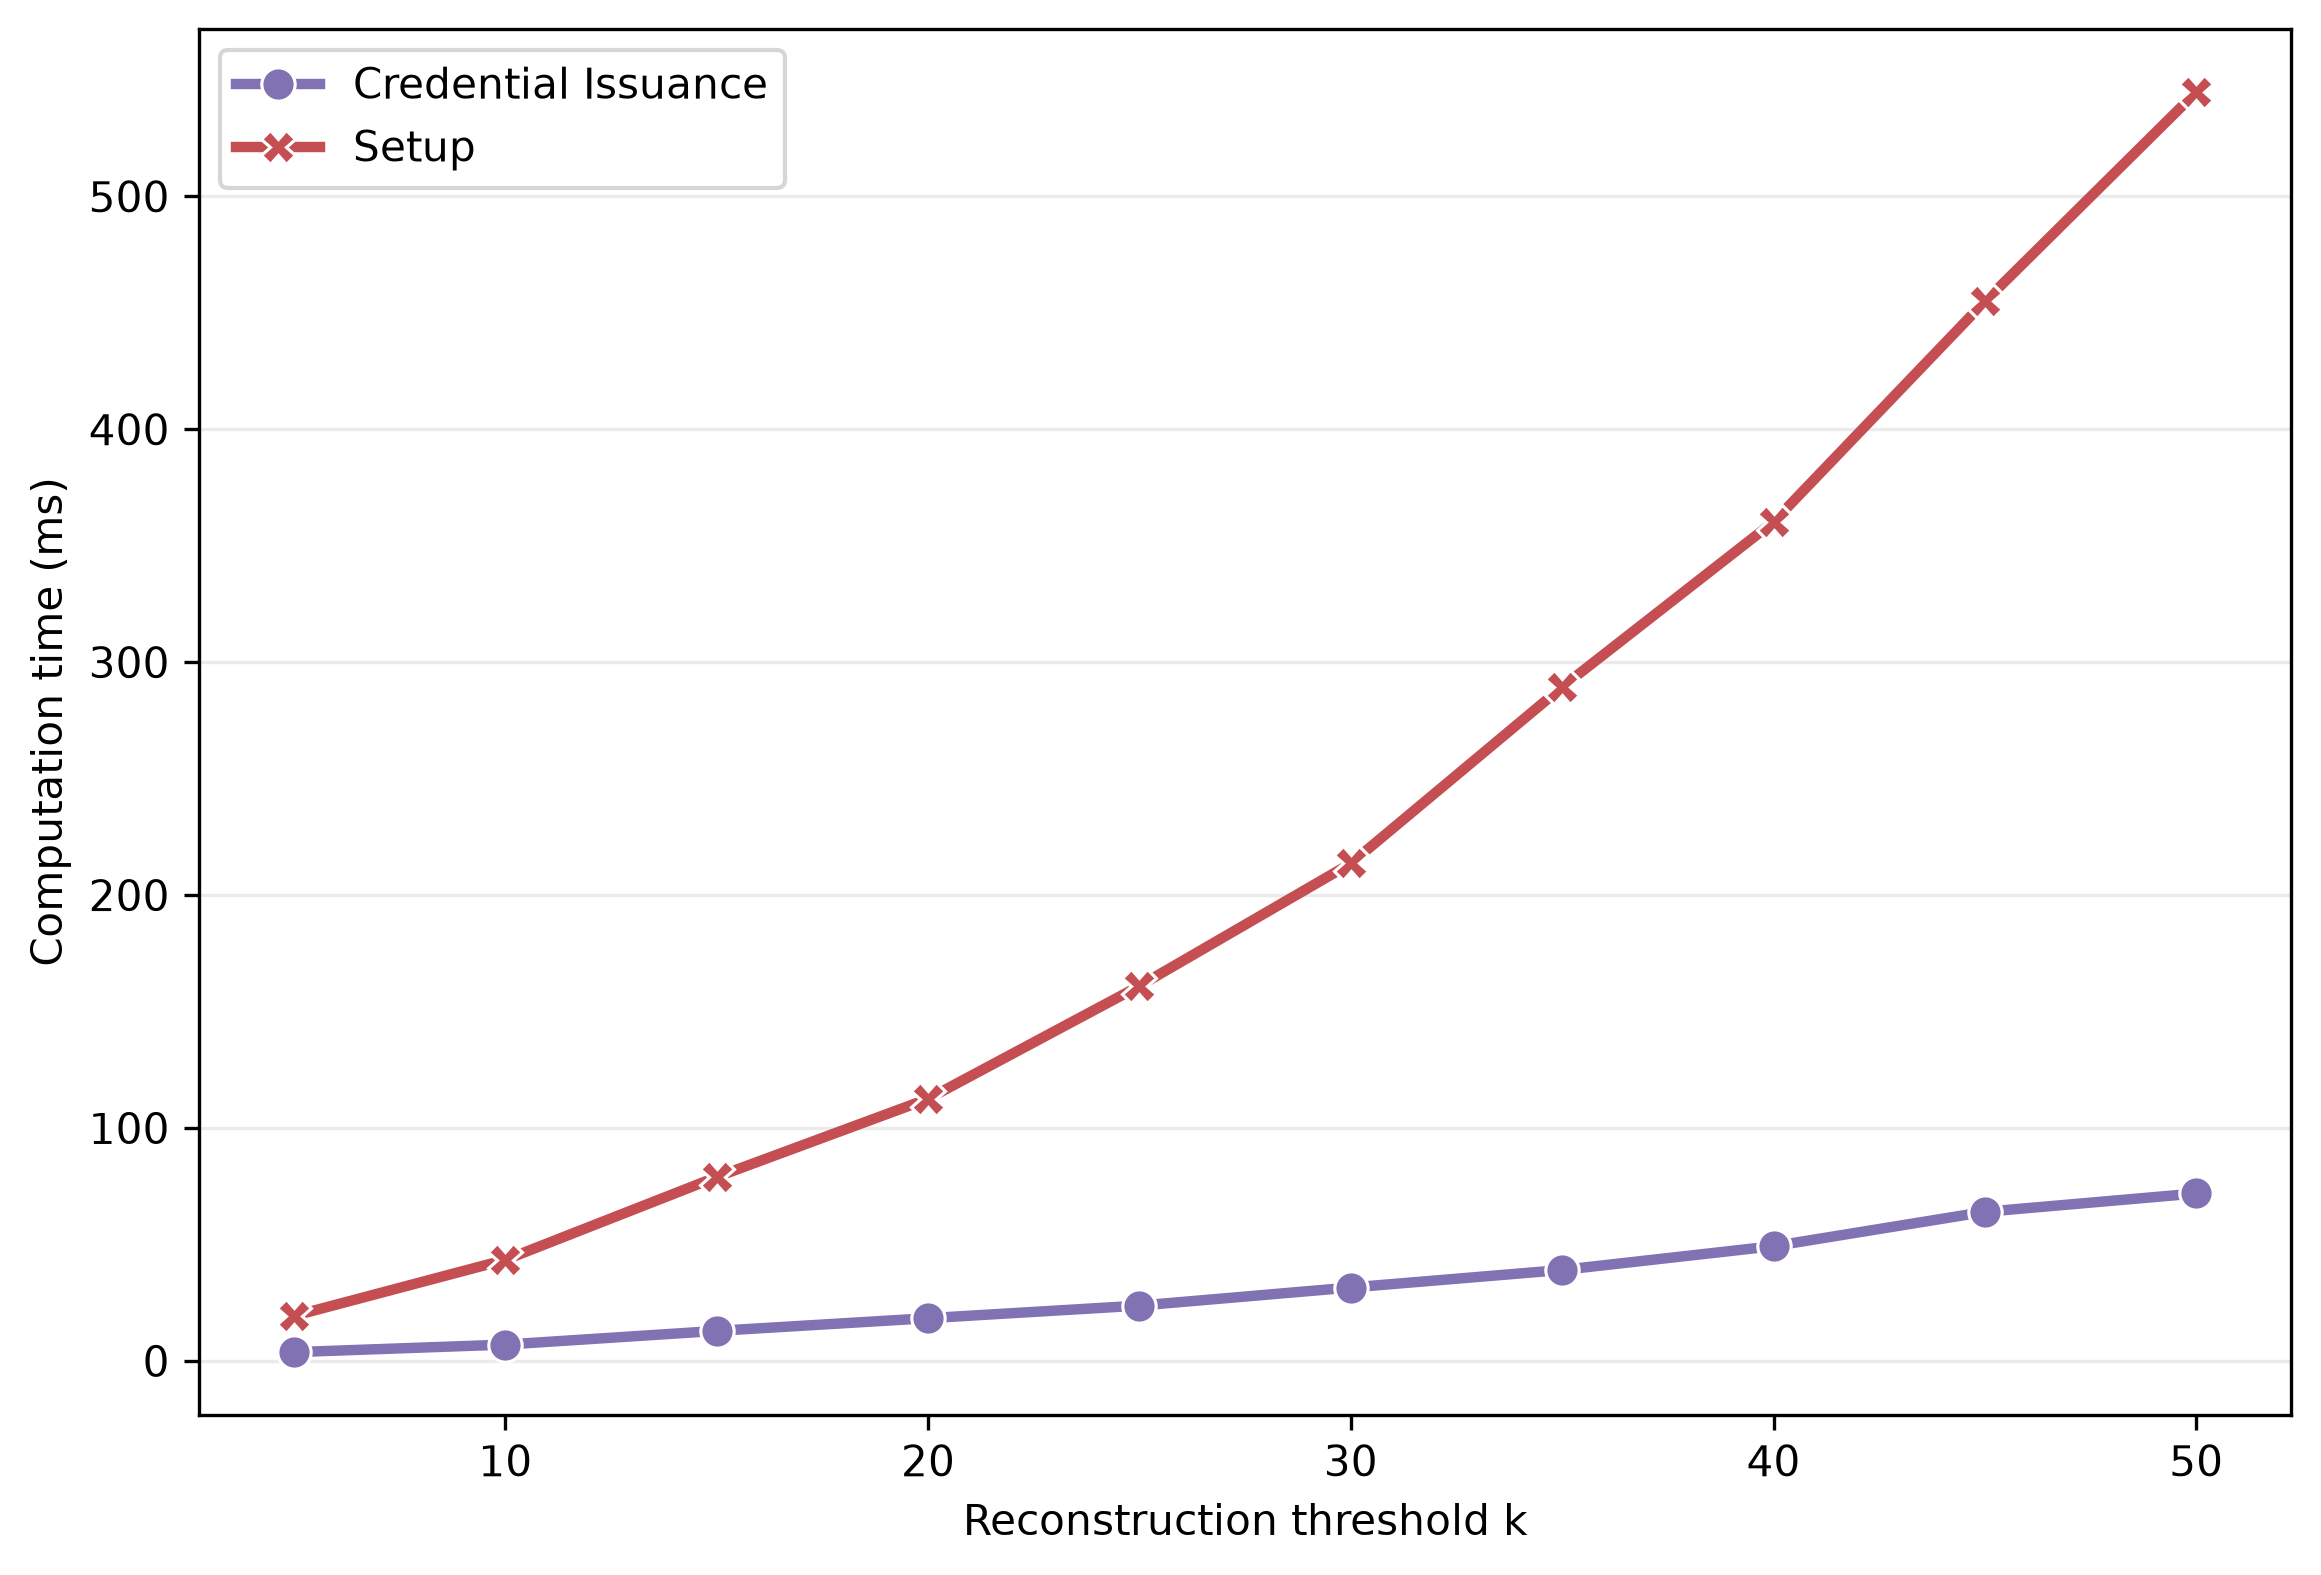
\includegraphics[width=\linewidth]{Images/setup.png}
    \caption{Computation time introduced by the setup procedure and by credential issuance as a function of the reconstruction threshold $k$.
    Setup is performed once, whereas credential issuance is performed by a client to obtain a destination-bound credential.}
    \label{im:setup_time}
\end{figure}



